%&tex
\documentclass{standalone}

\usepackage[dvipsnames]{xcolor}

\usepackage{tikz}
\usetikzlibrary{positioning,shadows}
\usetikzlibrary{arrows,chains,positioning,scopes,shapes.geometric,shapes.misc,shadows,decorations.markings}


\begin{document}

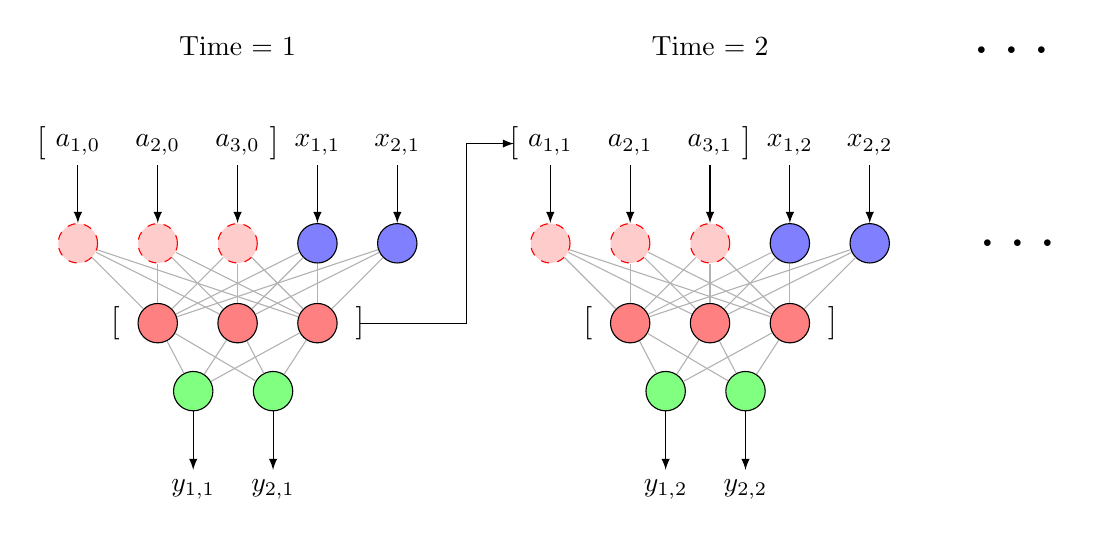
\begin{tikzpicture}

    % \draw[help lines, step=1cm,gray!20] (0,0) grid (10,-5);

    % input layer node
    \node[draw,
    circle,
    minimum size = 0.5cm,
    fill=blue!50] (x1_t1) at (0,0) {};
    \node[draw,
    circle,
    minimum size = 0.5cm,
    right = 0.5cm of x1_t1,
    fill=blue!50] (x2_t1) {};
    \node[draw,
    dashed,
    circle,
    color=red,
    minimum size = 0.5cm,
    left = 0.5cm of x1_t1,
    fill=red!20] (a3_t0) {};
    \node[draw,
    dashed,
    circle,
    color=red,
    minimum size = 0.5cm,
    left = 0.5cm of a3_t0,
    fill=red!20] (a2_t0) {};
    \node[draw,
    dashed,
    circle,
    color=red,
    minimum size = 0.5cm,
    left = 0.5cm of a2_t0,
    fill=red!20] (a1_t0) {};

    % hidden layer node
    \node[draw,
    circle,
    minimum size = 0.5cm,
    below = 0.5cm of x1_t1,
    fill=red!50] (a3_t1) {};
    \node[draw,
    circle,
    minimum size = 0.5cm,
    left = 0.5cm of a3_t1,
    fill=red!50] (a2_t1) {};
    \node[draw,
    circle,
    minimum size = 0.5cm,
    left = 0.5cm of a2_t1,
    fill=red!50] (a1_t1) {};

    % output layer nodes
    \node[draw,
    circle,
    minimum size = 0.5cm,
    below left = 0.5cm and 0.2cm  of a3_t1,
    fill=green!50] (y2_t1) {};
    \node[draw,
    circle,
    minimum size = 0.5cm,
    left = 0.5cm  of y2_t1,
    fill=green!50] (y1_t1) {};

    % drawing connectors
    \draw[color=black!30] (x1_t1) -- (a1_t1);
    \draw[color=black!30] (x1_t1) -- (a2_t1);
    \draw[color=black!30] (x1_t1) -- (a3_t1);
    \draw[color=black!30] (x2_t1) -- (a1_t1);
    \draw[color=black!30] (x2_t1) -- (a2_t1);
    \draw[color=black!30] (x2_t1) -- (a3_t1);
    \draw[color=black!30] (a1_t0) -- (a1_t1);
    \draw[color=black!30] (a1_t0) -- (a2_t1);
    \draw[color=black!30] (a1_t0) -- (a3_t1);
    \draw[color=black!30] (a2_t0) -- (a1_t1);
    \draw[color=black!30] (a2_t0) -- (a2_t1);
    \draw[color=black!30] (a2_t0) -- (a3_t1);
    \draw[color=black!30] (a3_t0) -- (a1_t1);
    \draw[color=black!30] (a3_t0) -- (a2_t1);
    \draw[color=black!30] (a3_t0) -- (a3_t1);
    \draw[color=black!30] (y1_t1) -- (a1_t1);
    \draw[color=black!30] (y1_t1) -- (a2_t1);
    \draw[color=black!30] (y1_t1) -- (a3_t1);
    \draw[color=black!30] (y2_t1) -- (a1_t1);
    \draw[color=black!30] (y2_t1) -- (a2_t1);
    \draw[color=black!30] (y2_t1) -- (a3_t1);

    \draw[latex-] (x1_t1) -- ++(0,1cm) node[above] {$x_{1,1}$};
    \draw[latex-] (x2_t1) -- ++(0,1cm) node[above] {$x_{2,1}$};
    \draw[latex-] (a1_t0) -- ++(0,1cm) node[above] {$a_{1,0}$};
    \draw[latex-] (a2_t0) -- ++(0,1cm) node[above] {$a_{2,0}$};
    \draw[latex-] (a3_t0) -- ++(0,1cm) node[above] {$a_{3,0}$};

    \draw[-latex] (y1_t1) -- ++(0,-1cm) node[below] {$y_{1,1}$};
    \draw[-latex] (y2_t1) -- ++(0,-1cm) node[below] {$y_{2,1}$};

    \node[above left= 0.75cm and 0.1cm of a1_t0](leftBracket1) {\large[};
    \node[above right= 0.75cm and 0.1cm of a3_t0](rightBracket1) {\large]};
    \node[above = 2cm of a3_t0] {Time = 1};

    \node[](Connector1) at (a3_t1.east){};
    \node[right = 0.5cm of x2_t1](Connector2){};

    \node[left= 0.1cm of a1_t1](leftBracket2a) {\large[};
    \node[right= 0.1cm of a3_t1](rightBracket2a) {\large]};

    \begin{scope}[shift={(6cm,0)}]
        % input layer node
        \node[draw,
        circle,
        minimum size = 0.5cm,
        fill=blue!50] (x1_t1) at (0,0) {};
        \node[draw,
        circle,
        minimum size = 0.5cm,
        right = 0.5cm of x1_t1,
        fill=blue!50] (x2_t1) {};
        \node[draw,
        dashed,
        circle,
        color=red,
        minimum size = 0.5cm,
        left = 0.5cm of x1_t1,
        fill=red!20] (a3_t0) {};
        \node[draw,
        dashed,
        circle,
        color=red,
        minimum size = 0.5cm,
        left = 0.5cm of a3_t0,
        fill=red!20] (a2_t0) {};
        \node[draw,
        dashed,
        circle,
        color=red,
        minimum size = 0.5cm,
        left = 0.5cm of a2_t0,
        fill=red!20] (a1_t0) {};

        % hidden layer node
        \node[draw,
        circle,
        minimum size = 0.5cm,
        below = 0.5cm of x1_t1,
        fill=red!50] (a3_t1) {};
        \node[draw,
        circle,
        minimum size = 0.5cm,
        left = 0.5cm of a3_t1,
        fill=red!50] (a2_t1) {};
        \node[draw,
        circle,
        minimum size = 0.5cm,
        left = 0.5cm of a2_t1,
        fill=red!50] (a1_t1) {};

        % output layer nodes
        \node[draw,
        circle,
        minimum size = 0.5cm,
        below left = 0.5cm and 0.2cm  of a3_t1,
        fill=green!50] (y2_t1) {};
        \node[draw,
        circle,
        minimum size = 0.5cm,
        left = 0.5cm  of y2_t1,
        fill=green!50] (y1_t1) {};

        % drawing connectors
        \draw[color=black!30] (x1_t1) -- (a1_t1);
        \draw[color=black!30] (x1_t1) -- (a2_t1);
        \draw[color=black!30] (x1_t1) -- (a3_t1);
        \draw[color=black!30] (x2_t1) -- (a1_t1);
        \draw[color=black!30] (x2_t1) -- (a2_t1);
        \draw[color=black!30] (x2_t1) -- (a3_t1);
        \draw[color=black!30] (a1_t0) -- (a1_t1);
        \draw[color=black!30] (a1_t0) -- (a2_t1);
        \draw[color=black!30] (a1_t0) -- (a3_t1);
        \draw[color=black!30] (a2_t0) -- (a1_t1);
        \draw[color=black!30] (a2_t0) -- (a2_t1);
        \draw[color=black!30] (a2_t0) -- (a3_t1);
        \draw[color=black!30] (a3_t0) -- (a1_t1);
        \draw[color=black!30] (a3_t0) -- (a2_t1);
        \draw[color=black!30] (a3_t0) -- (a3_t1);
        \draw[color=black!30] (y1_t1) -- (a1_t1);
        \draw[color=black!30] (y1_t1) -- (a2_t1);
        \draw[color=black!30] (y1_t1) -- (a3_t1);
        \draw[color=black!30] (y2_t1) -- (a1_t1);
        \draw[color=black!30] (y2_t1) -- (a2_t1);
        \draw[color=black!30] (y2_t1) -- (a3_t1);

        \draw[latex-] (x1_t1) -- ++(0,1cm) node[above] {$x_{1,2}$};
        \draw[latex-] (x2_t1) -- ++(0,1cm) node[above] {$x_{2,2}$};
        \draw[latex-] (a1_t0) -- ++(0,1cm) node[above] {$a_{1,1}$};
        \draw[latex-] (a2_t0) -- ++(0,1cm) node[above] {$a_{2,1}$};
        \draw[latex-] (a3_t0) -- ++(0,1cm) node[above] {$a_{3,1}$};

        \draw[-latex] (y1_t1) -- ++(0,-1cm) node[below] {$y_{1,2}$};
        \draw[-latex] (y2_t1) -- ++(0,-1cm) node[below] {$y_{2,2}$};

        \node[above left= 0.75cm and 0.1cm of a1_t0](leftBracket2) {\large[};
        \node[above right= 0.75cm and 0.1cm of a3_t0](rightBracket1) {\large]};

        \node[above = 2cm of a3_t0] {Time = 2};

        \node[above right = 2.1cm and 1cm of x2_t1] {\Huge$\dots$};
        \node[right = 1cm of x2_t1] {\Huge$\dots$};

        \node[left= 0.1cm of a1_t1](leftBracket2b) {\large[};
        \node[right= 0.1cm of a3_t1](rightBracket2b) {\large]};
    \end{scope}

    \draw (rightBracket2a.center) -| (Connector2.center);
    \draw[-latex] (Connector2.center) |- (leftBracket2.center);

\end{tikzpicture}

\end{document}
